% \documentclass{ipsjpapers}
\documentclass[draft]{ipsjpapers}

\input epsf
\input comment.sty

\usepackage{mediabb}
\usepackage[dvipdfm]{graphicx}

%% 巻数,号数などの設定
\setcounter{巻数}{50}
\setcounter{号数}{2}
\setcounter{volpageoffset}{1234}
\受付{20}{9}{17}
\採録{20}{11}{28}

% ユーザが定義したマクロなど.
\makeatletter
\let\@ARRAY\@array \def\@array{\def\<{\inhibitglue}\@ARRAY}
\def\<{\(\langle\)\nobreak}
\def\>{\nobreak\(\rangle\)}
\def\|{\verb|}
\def\Underline{\setbox0\hbox\bgroup\let\\\endUnderline}
\def\endUnderline{\vphantom{y}\egroup\smash{\underline{\box0}}\\}
\def\LATEX{\iLATEX\Large}
\def\LATEx{\iLATEX\normalsize}
\def\LATex{\iLATEX\small}
\def\iLATEX#1{L\kern-.36em\raise.3ex\hbox{#1\bf A}\kern-.15em
    T\kern-.1667em\lower.7ex\hbox{E}\kern-.125emX}
\def\LATEXe{\ifx\LaTeXe\undefined \LaTeX 2e\else\LaTeXe\fi}
\def\LATExe{\ifx\LaTeXe\undefined \iLATEX\scriptsize 2e\else\LaTeXe\fi}
\def\Quote{\list{}{}\item[]}
\let\endQuote\endlist
\def\TT{\if@LaTeX@e\tt\fi}
\def\CS#1{\if@LaTeX@e\tt\expandafter\string\csname#1\endcsname\else
	$\backslash$#1\fi}


%\checklines	% 行送りを確認する時に使用
\begin{document}%{
% 和文表題
\title[分散OS開発学習キット LP49]  %
	{分散OS開発学習キット LP49}
% 英文表題
\etitle{An open source kit for developing and studying a distributed OS ``LP49''}

% 所属ラベルの定義
\affilabel{NII}{国立情報学研究所\\NII}
\affilabel{Hitachi}{日立製作所\\Hitachi}
% 和文著者名
\author{丸山 勝巳\affiref{NII}\affiref{NII}\and
	佐藤 好秀\affiref{NII}}
	
% 英文著者名
\eauthor{Katsumi Maruyama\affiref{NII}\affiref{Princeton}\and
	Yoshihide Sato\affiref{NTT}\affiref{Hitachi}}

% 和文概要
\begin{abstract}

% 行く川の流れは絶えずして\\
% しかももとの水にあらず.\\
% 淀みに浮かぶうたかたは\\
% かつ消えかつ結びて久しくとどまりたることなし。\\


 
\end{abstract}

% 英文概要
\begin{eabstract}
  Control systems (e.g. embedded systems, home servers) are becoming more and more sophisticated, 
networked and complex. 
Software productivity and dependability are the first concern of their design. 
OS’s for control systems must support distributed processing, 
fail-robustness and ease of program development. 
LP49 is a component-oriented OS with micro-kernel and multi-server architecture. 
We have adopted the L4 micro-kernel because of its performance and flexibility. 
Plan 9 had devised excellent distributed processing facilities 
(e.g. 9P protocol, private name space, user-mode servers), 
and we have largely adopted concepts and source code from Plan 9. 
LP49 component architecture will be effective to improve dependability.

\end{eabstract}

% 表題などの出力
\maketitle

%}{

% 本文はここから始まる
\section{はじめに}

 今や組み込みシステムやホームサーバには、NW接続された多様な機器を連携動作させる
分散処理機能が必須である。
OSはシステムの性能(機能・効率・信頼性)のみならず
プログラム開発コスト(開発しやすさ、開発期間・拡張性など)を大きく左右する。
信頼性向上の近道はシンプル化であり、
目的に最適な分散OSを作りたい人にはシンプルな分散OS開発キットは意義がある。

  また、OSはソフトウェア技術の集大成であり、最高のソフトウェア教材である。
学習用OSは、重要機能を含み、構成が簡明で、容易に機能追加でき、
プログラム規模も小さいことが望まれる。
学習用OSとしては、Minix が大変すぐれているが、
残念ながら分散処理機能は目的としていない。

このように、分散OSの適切な開発学習キットは大変意義が高い。
本報告は、以上の観点から分散OS開発学習キットLP49について紹介する。


%}{

\section{本OS開発学習キットの意図}\label{sec:Enum}\label{sec:item}

シンプルな分散OS開発学習キットに向けて、以下を行っている。

\begin{description}

\item[組込みシステムに適したシンプルなOS]
    組み込みシステムに必要な機能をもったコンパクトなOS。
    
\item[耐障害性]
    部分障害が生じても、システムクラッシュせず、
    障害部分だけの再開でサービスを継続できるようにする。
    このためには、マイクロカーネル+ユーザモードのマルチサーバ構成とする。
    
\item[拡張性の強化]
    機能追加は、OSカーネルを修正せず、できるだけ外付けプログラムで行えるようにする。
    
\item[分散処理・連携機能]
      分散リソースの融通性の高い管理と制御、
      別ノードの名前空間の可視化、実行環境の連携、
      などを実現する。
    
\item[プログラム開発の容易化]
    カーネルモードプログラムは開発が困難である。
    マイクロカーネル以外は、デバイスドライバも含めてユーザモード化する。
    
\item[L4とPlan9のソースコード活用]  
     OS全体をスクラッチから作るには、膨大な工数を要する。
    Karlsruhe大学の L4 マイクロカーネルは、 
    簡潔で優れたスレッド・メッセージ性能を持っている。
    また、Bell研で開発された Plan9 は、融通性の高い分散処理を実現している。
    かつ両者ともオープンソースであるので、ソースコードを活用して
    工数削減をはかった。
    
\item[使い慣れたプログラム開発環境]
  特別な環境が必要では敷居が高い。
    使い慣れたGNU環境でコンパイルからテスト走行まで出きるようにする。

\end{description}    


%}{

\section{基本発想}

\subsection{マイクロカーネル}

   OSの疎結合モジュール化、デバイスドライバを含むプログラムのユーザモード化、
  個別プロセス再開による耐障害強化、マルチスレッドプログラミングの容易化の観点から
  マイクロカーネル型OSとした。
  マイクロカーネルは、スレッドとメッセージの性能が優れ、かつシンプルな
  L4 を利用した。

\subsection{マルチサーバー構成}
 
 OS全体を管理するモジュールは、L4マイクロカーネルの1タスク(論理空間+スレッド)として
  ユーザモードで実行させている。
  これを ``LP49-CORE'' と呼ぶ。 


\subsection{すべてのリソース・サービスをファイルトリーとして扱う}

   Unixでは、すべてのリソースが階層的ファイルトリー上に名前付けされており(名前空間)、
  ファイルとしてアクセスできることを目指したが、
  この理念はネットワーク(NW)を始めとして早期に破綻した。
  LP49 では Plan9 を踏襲して、NWも含めてすべてアクセス対象を
  名前空間(ディレクトリー)上の名前で識別でき、
  ファイルインタフェース(open(), read(), write(), 等) で操作されるオブジェクト
  として扱っている。
  つまり、Plan9/LP49 では、
  一般のファイルシステムのみならず全てのリソースやサービスも、
  操作法はファイルシステムとして統一されており、
  各々の名前空間を有している。 

\begin{comment}
  例えば, インターネットサービスは以下の様にディレクトリを形成している。
  ここに /tcp/0, /tcp/1,,, は個々のコネクションを表す。

{\footnotesize
\begin{verbatim}
        --+-- tcp/ -----+-- clone                               
          |             |-- stats                       
          |             |-- 0/ ---+-- ctl                
          |             |         |-- data          
          |             |         |-- local         
          |             |         :
          |             |
          |             |-- 1/ ---+-- ctl                
          |             |         |-- data          
          |             :         |-- local         
          |                       :
          |                
          |-- udp/ -----+-- clone                             
          |             |-- stats                       
          |             |-- 0/ ---+-- ctl                
          |             |         |-- data          
          |                       |-- local         
          |                       |                
          |--- arp/ ----
          :
\end{verbatim}
}
\end{comment} 



\subsection{サービス部品:サーバとサーバント}

  OSが提供するサービスには、
  DOSファイルサービス、EXT2ファイルサービスといった高位サービスと、
  ハードウェア駆動、モジュール間通信、NW接続、サーバ登録簿といった低位サービス
  とがある。

  前者は、個々に独立性が高く、規模も大きくなりがちなので、
  サービス毎にユーザモードで走るプロセスとして実現する。これを{\bf サーバ}と呼ぶ。
  サーバはメッセージインタフェースなので、ローカルでもリモートでも同等に使える。
  ユーザモードプロセスなので、プログラム開発の容易化のみならず、
  障害時もそのサーバだけを停止・再開することで耐障害性も強化される。

  後者は、共通部品的であり、より実行速度が重視されるので、
  独立したプロセスとはせず LP49-CORE内のモジュールとして実装することとした。
  このモジュールを{\bf サーバント}と呼んでいる。
  サーバントは、統一インタフェースを持つコンポーネントである。
  機能的には、同一サービスをサーバで実装することもサーバントで実装することも可能である。


\subsection{マルチサーバと9Pプロトコル}

  サーバのプロトコル(メッセージインタフェース)は、
  サーバが提供できる機能と性能を決定する。
  独自プロトコルは、いくら強力であっても普及させることは至難である。
  Plan9の{\bf 9Pプロトコル}は、
  {\tt attach(), walk(),open(), create(), 
  read(), write(), clunk(), remove(), stat(), wstat() }
  等のメッセージからなり、
  低レベル制御も可能で融通性が高いので、これを採用した。
  9Pプロトコルを採用した副産物として、少ない修正で
  Plan9のサーバをLP49に移植することも可能になった。


\subsection{名前空間とその接続}

  前述のように、サーバもサーバントもリソースはファイルとして抽象化されており、
自分の名前空間を持つので、UNIXでいうファイルシステムである。

図 \ref{fig:NS-server-servant} に示すように、
ルートファイルシステム({\bf RootFS}: 実はこれもサーバント)を出発点とする{\bf 名前空間}に、
サーバやサーバントを接続(マウント)することにより、プロセスに見えるようになる。
``/dev'' には各種デバイスサーバントが、``/net''にはプロトコルスタックが接続されている。
サーバはリモートの可能性もあるので、マウントの仕組みは後で説明する。

\begin{figure}[htb]
  \begin{center}
   \epsfxsize=400pt
   \epsfbox{fig/NS-server-servant.eps}
    \caption{サーバ、サーバントと名前空間}
    \label{fig:NS-server-servant}
  \end{center}
\end{figure}



\subsection{プロセス個別名前空間}

  UNIXではファイルシステムの mount は root のみが行え、
  名前空間は全プロセスで共通である。
  これに対し、Plan9/LP49 の名前空間は、
  各プロセス毎に自前の名前空間({\bf 個別名前空間})を持つことができる。
  名前空間はアクセス保護の役目を持つので、緻密なセキュリティー管理を
  実現できる。



%%%
\section{本OSの構造 概要}\label{sec:ITEM}

\subsection{階層構造}
      図 \ref{fig:LP49general} に示すように、
  LP49 は以下の階層からできている。
    
\begin{figure}[htb]
  \begin{center}
   \epsfxsize=400pt
   \epsfbox{fig/LP49general.eps}
    \caption{LP49全体構成}
    \label{fig:LP49general}
  \end{center}
\end{figure}


\begin{enumerate}
\item   L4マイクロカーネル  \\
    L4マイクロカーネルが、スレッド制御、タスク空間(プロセス相当)制御, 
    スレッド間通信、ページ制御、割り込み検出と通知を行っている。
    マイクロカーネルのみがカーネルモードで走り、それ以外は
    デバイスドライバも含めてユーザモードで走る。

    
\item  HVM \\
    LP49 のスタートアップと、page-faultを処理するページャー (Pager) スレッド 
    の機能を持っている。
    将来、VM機能を追加して Hypervisor Module 化する予定で、HVMと名づけた。

\item  LP49-CORE \\
    応用プログラム(以下APLと呼ぶ)のシステムコールを受けて, 
    適切なサーバやサーバントに処理を行わせる。 
    ネットワークサービスや、デバイスドライバも含まれる。
    
\item  サービス階層 \\
    OSサービスを行うサーバー類も普通の応用プログラム(APL)も、
    同等のユーザモードプロセスである。
    サーバは、9Pプロトコルを喋れる APLである。
\end{enumerate}    

%}{


%%%%%
\subsection{サーバント}

   サーバントはハードウェアデバイス, サーバ登録簿、環境変数記憶、
pipe, プロトコルスタックなど低位サービスを提供する。
サーバントはLP49-COREプロセス内のモジュールであり、
attach(), init(), open(), read(), write(),,, といったプロシージャインタフェース
で呼ばれる。


\begin{figure}[htb]
\begin{center}
{\tiny
\begin{verbatim}
         *-----------------------------------------------------------------*  
         |  *-interface-* *--------*      *----------* *----------*        |  
         |  | type      | |  init  |      | open     | |  read    |        |  
         |  | name      | |  func  |      |  func    | |  関数    |        |  
         |  | (*init)() | |        |      |          | |          |        |  
         |  |    :      | |        |....  |          | |          |......  |  
         |  | (*open)() | |(static |      | (static  | | (static  |        |  
         |  | (*read)() | |  func) |      |   func)  | |   関数)  |        |  
         |  | (*write)()| |        |      |          | |          |        |  
         |  |   :       | |        |      |          | |          |        |  
         |  *-----------* *--------*      *----------* *----------*        |  
         *-----------------------------------------------------------------*  
\end{verbatim}
}
\caption{サーバントの構造}
\label{fig:servant}
\end{center}
\end{figure}


  サーバントもいわゆるファイルシステムであり、自分の名前空間をもつ。
  つまり、
  サーバント内の各要素はディレクトリ(つまり名前空間)で名前付けされており、
  ファイルインタフェースで操作できる。
  サーバントは \verb|#+<英字>| の形式のサーバント名をもつ。
  代表的サーバントを以下に示す。括弧内は サーバント名である。

{\small
\begin{verbatim}
     コンソール (#c), ハードディスク (#S), フロッピーデバイス(#f), 
     環境変数 (#e), サーバ登録簿 (#s), Remote Procedure Call (#M), 
     Etherドライバ (#l), プロトコルスタック (#I), Pipe (#|), 
     ルートファイルシステム (#R), USBホストコントローラ (#U), 
     VGAコントローラ (#v)、   ...

\end{verbatim}
}

``bind''コマンドにより、サーバントをプロセスの名前空間に結合することにより、
プロセスからサーバントにアクセスできるようになる。

  \verb|    bind [-abc]  サーバント名  マウントポイント|  \\



\subsection{サーバ}

  サーバはサービスごとに独立したユーザモードのプロセスであり、
  9Pメッセージ (9Pプロトコル)を受信してサービスを実行する。
  LP49-COREとサーバの間で9Pメッセージを運ぶ接続を{\bf サーバリンク}と呼んでいる。
  サーバリンクは、
  ローカルサーバの場合は pipe (LP49の pipe は 双方向である)、
  リモートサーバの場合は TCP/IP 接続を用いる。

  サーバは自分のサーバリンクを``サーバ登録簿''に登録しておく。
  サーバ登録簿はサーバントの一つ(\#s)で、 立ち上げ時に ``/srv``
 として接続されている。
  クライアントは、サーバ登録簿から目的のサーバを見つけて、
  サーバリンク名(ex. /srv/dos) を自分の名前空間にマウントする。
  これにより、サーバの名前空間がクライアントの名前空間に接続され、
  普通のファイルインタフェースでアクセスできるようになる。

  \verb|    mount [-abc]  サーバリンク名  マウントポイント  場所 |  \\


%%%%
\subsection{システムコールの仕組み}

  モノリシックOSでは、APLのシステムコールはトラップを使ってOSカーネルに飛び込むのに対し、
本OSのシステムコールは、APLからLP49-COREへのメッセージ通信となる。
  システムコールの仕組みを、図 \ref{fig:LP49syscall}に示す。

{\bf (1) ライブラリによるL4メッセージ化}

   APLのシステムコールは, 使い慣れた関数呼び出し (open(...), read(...), write(...),,,) 
  である。
  ライブラリは、これを L4 メッセージに変換して LP49-CORE に送り、返答メッセージを待つ。
  APLとLP49-COREは別論理空間なので、アドレス引き継ぎは使えない。
  システムコールの引数は、L4メッセージの値コピー, 
  バッファー域はL4メッセージのページマップ機能を使って引き継いでいる。


{\bf (2) LP49-CORE マルチスレッドサーバ}

    LP49-COREの位置付けは、プロセスに対してはサーバであり、
    サーバプロセスに大してはクライアントといえる。

    システムコールの処理は中断が生じうる。
    複数のAPLからの要求を並行して処理するために、
    マルチスレッドサーバを実装した。

    要求メッセージはMngrスレッドに送られる
    (L4メッセージの宛先はスレッドである)。
    Mngrスレッドは、スレッドプールから空きclerkスレッドを
    割り当てて、それに処理を行わせる。


{\bf (3) サーバントアクセスの仕組み}
  
    システムコールの対象がサーバントである場合は、
    図 \ref{fig:LP49syscall}に示すように clerkスレッドが
    サーバントの関数を呼び出す。


{\bf (4) サーバアクセスの仕組み }

    システムコールの対象がサーバである場合は、
    図 \ref{fig:LP49syscall}に示すように
    clerkスレッドは {\bf マウントサーバント} を呼ぶ。
    マウントサーバント(\#M)はサーバをマウントするための仕組みであり、
   システムコール引数から9Pメッセージを編集して、
    目的サーバがノード内の場合は Pipeサーバント,
    別ノードの場合は TCPコネクションを経由して、Remote Procedure Callを行う。


\begin{figure}[htb]
  \begin{center}
   \epsfxsize=340pt
   \epsfbox{fig/LP49syscall.eps}
    \caption{システムコール}
    \label{fig:LP49syscall}
  \end{center}
\end{figure}


%%%
\subsection{Pagerの仕組み}

  LP49のプロセスは論理空間で保護されている。
  L4マイクロカーネルでは、スレッドの実行中にpagefaultが生じると、
  登録されている{\bf Pager}スレッド にPagefaultメッセージが送られる。
  Pager は L4ユーザがプログラムできるスレッドであり、
  Pagefaultメッセージの引数を見て適切なページをマップするなど、
  自前の論理を組み込むことができる。
  L4スレッドは、生成時に Pager を指定しておく。

  Pager は pagefault メッセージに応じたメモリマップを考えて
  L4のmap機能を行うだけの普通のスレッドである。
  LP49 の 通常の Pagerは HVM 階層に含まれているが、
  LP49ユーザが独自 Pager を追加することも可能である。

  現在の Pager は基本機能のみ実現しているが、
  Pager は大変融通性に富んでおり、
  Pagerの機能強化により次のような色々な展開が可能である。


\begin{itemize}
\item[ページキャッシュ]  .....

\item[トランザクションメモリ]  ....

\item[共用メモリ] ....

\item[性能向上]  ....
\end{itemize}



%%%
\section{分散処理と名前空間}
\subsection{名前空間の機構}

名前空間の構成法を図 \ref{fig:NSmount} に示す。
LP49-COREは、ルートファイルシステム(RootFS)を有している。
図中の(a)では、
サーバントをRootFSの適当なマウントポイントに
結合 (bind) することにより、
サーバントの名前空間がホストの名前空間に接続され、
サーバントのサービスを受けられるようになる。
サーバントは、procedure callで呼び出されるので、自ホスト内に限られる。

同様に(b)では、サーバーをマウント (mount) することにより、
サーバの名前空間がホストの名前空間に接続され、  
サーバのサービスを受けられるようになる。    
サーバは remote procedure call で呼び出されるので、
自ホスト内(b)でもリモートホスト上(c)でも、
まったく同様にアクセスできる。

また、マウントはサーバ単位だけではなく、
図 \ref{fig:NSmount}-(d)のremote-host の名前空間の"部分名前空間"を別のホストの
マウントポイントにマウントすることも可能である。
この仕組みについては、後で説明する。


\begin{figure}[htb]
  \begin{center}
   \epsfxsize=340pt
   \epsfbox{fig/NSmount.eps}
    \caption{名前空間とマウント}
    \label{fig:NSmount}
  \end{center}
\end{figure}



%%%
\subsection{サーバ登録簿とサーバのマウント}

前述のように、サーバとLP49-COREの間で 9Pメッセージを運ぶ接続がサーバリンクである。
サーバリンクは、ローカルサーバの場合はpipe, リモートサーバの場合は TCP/IP接続
である。

  サーバ登録簿は ``\#s'' という名前のサーバントであり、
  初期設定により名前空間の ``/srv'' に接続されている。
  各サーバは、サーバリンクをサーバ登録簿サーバント (/srv/*) に登録する。
  例えば EXT2ファイルサーバは、``/srv/ext2''というファイルを作って、
  そこにサーバリンクのfile descriptor を書き込んでおく。


  クライアントは、サーバ登録簿から目的のサーバを見つけて、
  これを自分の名前空間にマウントすることで、
  サーバの持つ名前空間にアクセスできるようになる。\\

\begin{verbatim}
  [例]    mount -a /srv/dos /c /dev/sdC0/dos 
\end{verbatim}

これは、DOSファイルサーバ (``/srv/dos'')を使って、
HDD (``/dev/sdC0'')のDOS partition を
``/c'' にマウントしている。


\subsection{プロトコルスタック}

    NW (network)機能は OS の最重要機能の一つであり、OS技術者/研究者は 
  プログラム構造とロジックを完全にマスターしておくべきである。
  Plan9 のNWプログラムは, 
  stream, xkernel などの研究成果が反映され簡明である、
  Plan9 用に開発されたEtherドライバを少ない修正で流用できる、
  ことから、LP49 は基本的に Plan9 を継承している。

  ネットワーク関連のプログラム構成を、図 \ref{fig:NWservants} に示す。
  IPサーバント(``\#I'')を介して、TCP, UDP, IP など各プロトコル毎にモジュール化された
  プログラムが動作している。
  IPサーバントは Internet サービスのインタフェースであり、
  ユーザには以下のトリー構成をもつファイルシステムとして見える。
 IPサーバントは普通 ``/net''に接続するので、``/net/tcp''はTCPを, 
  ``/net/udp''はUDPを意味する。
  個々の接続も名前空間に現れ、
  例えば /net/tcp/0, /net/tcp/1 ,,, は、TCP接続を表す。



{\footnotesize
\begin{verbatim}
        --+- tcp/ ----+- clone                        
          |           |- stats                
          |           |- 0/ ---+- ctl          
          |           |        |- data     
          |           :        |- local    
          |                    |           
          |- udp/ ---+- clone                        
          |          |- stats                  
          |          |- 0/ ---+- ctl            
          |          |        |-data     
          |          :        |-local    
          |                   |           
          |- ipifc/ -----+- clone                         
          |              |- stats                   
          |              |- 0/--                    
          |              |                          
          |-- ndb/ ----                                   
          |                                              
          |-- arp/ ----
\end{verbatim}
}


Etherサーバント(\#l)は、 Ether card のサービスインタフェースであり、
該当した Ether driver を呼び出している。


\begin{figure}[htb]
  \begin{center}
   \epsfxsize=420pt
   \epsfbox{fig/NWservants.eps}
    \caption{IPサーバントとEtherサーバント}
    \label{fig:NWservants}
  \end{center}
\end{figure}


%%%%%%%%%%%
\subsection{名前空間のexport/import}

  
リモートホストの名前空間の``部分''名前空間を
マウントすることも可能である。
図 \ref{fig:NSmount} の(d)は、リモートホストの部分名前空間をマウントしている
例である。

例えばリモートホストの /dev ディレクトリーをローカルホストにマウントすると、
/dev に接続されているリソースにアクセスすることが可能になる。
全てのオブジェクトはファイルインタフェースで操作できるので、
このことはリモートホストのデバイスも操作できることを意味する。


同様にして、Plan9ユーザグループから移植した U9FS というプログラムを
Unix上で走らせることにより、
UNIXのファイルシステムの部分空間を LP49 上にマウントすることも可能である。





%}{

\section{LP49とPlan9の対比 }

LP49では、Plan9の財産をできる限り活用するようにしたが、
実施してみるとかなりの修正を必要とした。(表 \ref{table:LP49-Plan9})

{\bf (1) 構造の違い}

L4を使ったマイクロカーネル構造にしたため、
マルチスレッドサーバ化、
システムコール,
....

{\bf (2)言語仕様/開発環境の差}

Plan9 は、独自拡張されたC言語で書かれている。
特に構造体の無名フィールド (フィールド名を省略でき、
その場合コンパイラがデータタイプから目的フィールドを
自動的に探す)が多用されている。


{\bf (3) サーバとドライバ}

サーバとドライバプログラムは、Plan9 から少しの修正で移植が可能だった。

\begin{table}[htb]
\caption[Plan9vsLP40]{LP49とPlan9の対比 }
\label{table:LP49-Plan9}
\begin{center}
{\footnotesize 
\begin{tabular}{|l|l|l|}
\hline
 分類  & Plan 9 & LP49 \\
\hline

Micro kernel  &     No        &   Yes   \\
\hline

並行処理  &  プロセスはコルーチン、 &   L4 Process  \\
          &  スレッドはメモリ域共用のプロセス &  L4 Thread \\
\hline

システムコール    & Trap       &     L4 メッセージ \\
                  & カーネル+ユーザプロセス    & マルチスレッドサーバ \\
\hline

〃データ入力      & Plan9カーネルが   & L4ページマップ \\
〃データ出力      & APL空間を直接アクセス          & L4 ページマップ \\
\hline

ドライバ     & カーネルモード    & ユーザモード  \\
\hline

言語仕様 &  Plan9独自のC                     &   GCC   \\
         &  無名フィールド, 無名パラメータ   & \\
         &  typedef, USED(), SET()           &    \\
         &   \#pragma, 自動ライブラリリンク  & \\
\hline

コンパイラ  &   Plan9 独自Cコンパイラ   &   GCC \\
\hline

 Utility  &  Plan9 の Linker, Assembler, mk    & GCC, gld, gmake \\
\hline

Binary    &  a.out形式         &    ELF形式 \\
\hline

\end{tabular}
}
\end{center}
\end{table}


%}{
\section{本OSキットの開発環境展}

OSの開発および学習には、使い慣れた開発環境が望まれる
(Plan9が普及しない理由は独自の開発環境にもある)。
またOSの走行テストも、NW機能を含めて実機の前に仮想マシンで行えることが望まれる、

LP49の開発環境を図 \ref{fig:SDE}に示す。
LP49のプログラム開発は、Linuxホスト上の GNUツールだけで行っている。
LP49の走行テストは、オープンソースエミュレータ QEMU の中で行っている。
QEMU はネットワーク機能も提供しており、1台のホストマシンの上で、
LP49-LP49 通信、LP49-Linux通信などを行える。
1台のホストマシン上で、コンパイルからNWを含む走行試験まで
時間を待たずに(make clean; make; から LP49立ち上げまで40秒)できることは、
非常に好都合である。


\begin{figure}[htb]
  \begin{center}
   \epsfxsize=360pt
   \epsfbox{fig/SDE.eps}
    \caption{開発試験環境}
    \label{fig:SDE}
  \end{center}
\end{figure}


%}{
%%%%%
\section{本OSキットによる展開例}

\subsection{ソフトウェアバス}

LP49では、OSサービスはサーバもしくはサーバントによって提供される。
LP49-COREは、サーバント・サーバのマルチプレクサ、もしくは
APLとサーバやサーバとの間を連携させるメッセンジャーに徹しており、
これがシンプル化に役立っている。
ただし、現方式ではシステムコールは全て LP49-CORE を経由して処理されるが、
目的サーバが決まってしまえば、
APLとサーバの間で直接メッセージをやり取りさせることもできるで、
更なる簡潔化が可能である。
具体的には、目的サーバの決定に関わるopen(), create(), chdir()、close() を
LP49-COREが処理してAPL-サーバ間を安全なチャンネルで接続させる。

また、9Pプロトコルは同期型メッセージであるが、
非同期型メッセージもサポートすることにより、
広域分散をより効率的に行うことも可能と思われる。
非同期メッセージの拡張として、サーバを関数型言語 Erlang で実装することも
考えられる。


\begin{comment}
図 \ref{fig:simpleOS}

\begin{figure}[htb]
  \begin{center}
   \epsfxsize=400pt
   \epsfbox{fig/simpleOS.eps}
    \caption{簡明なOS構成}
    \label{fig:simpleOS}
  \end{center}
\end{figure}
\end{comment}


\subsection{耐障害強化}

プロセスを監視し、障害が見つかればそれを停止して再スタートする仕組みを
容易に組み込める。
また、簡単なPagerの機能追加により、プロセスに保持メモリ域を追加することができる。
保持メモリ域には、プロセスが指定した適当なタイミングで
無矛盾なデータのスナップショットを書き込んでおく。
プロセスが障害になった場合には、保持メモリ域のデータを使って再開させることにより、
比較的安全なroolbackを行える。

Cf. Minix-3, Erlang



\subsection{高性能化}
 
現 LP49 には、高性能化の仕組みはほとんど組み込んでない。
スレッドの優先度、システムコールの引数引き継ぎ等、容易に高性能化を
図ることができる。
また、Pager に機能追加をすることで、容易にページキャッシュを実現することも可能である。



\subsection{認証システム}

分散OSにおいて認証は非常に重要な課題である。

Plan9はKerberos を拡張した精妙な認証方式を実装しているが、
学習用としては複雑である。

LP49では,
Identity-Based Encryptionを使用した認証方式を検討する予定である。


% \begin{figure}[t]
% 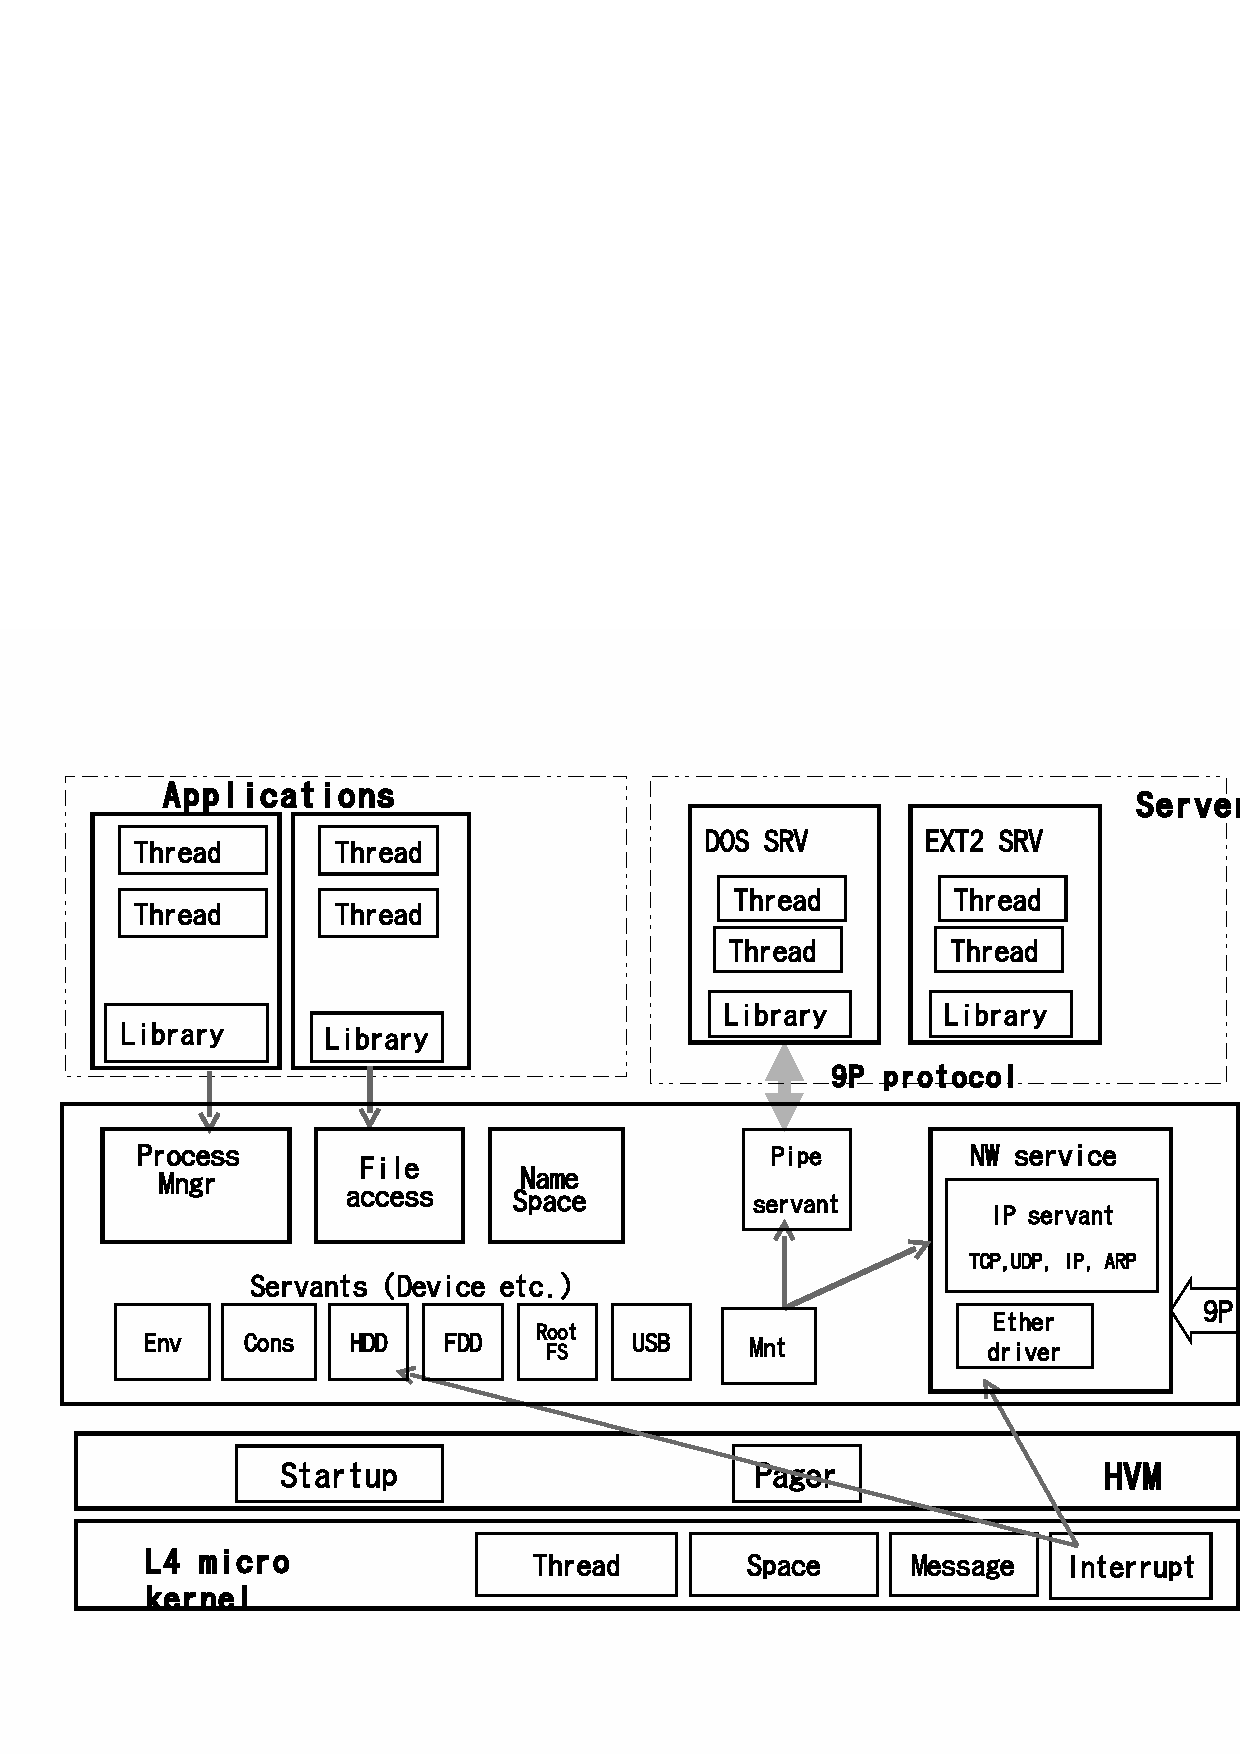
\includegraphics[width=7.5cm]{fig/LP49general.pdf}
% \caption{隣接通信の実行時間}
% \label{fig:fig/LP49general}
% \end{figure}


\section{関連研究}

{\bf L4}


{\bf Plan9} 

{\bf Minix} は学習用マイクロカーネルOSとして、非常に意義が高い。
LinuxはMinixから影響を受けて開発されたが、マイクロカーネルは採用されなかった。
個人でOSを作るには、全てのカーネルデータが見えるモノリシックOSの方が
作り易いし効率も良いというLinusの主張に一理はあるが、
障害にたいする頑強性、プログラム保守性はマイクロカーネルが有利である。
Minix は分散OSとしての機能は範囲外である。






{\bf SawMil}はIBM で実施されたL4 マイクロカーネルと
マルチサーバからなるOS の研究プロジェクトである。
Linux カーネルをサービス対応にモジュール分けしてマルチサーバ化することを
狙ったが、Linuxカーネルはモジュール分割が困難のため、
プロジェクトは中第した。

{\bf $L^4Linux$}は、L4 マイクロカーネルの上でLinux を動かすOSである。
Linux はモノリシック構成のままであり、L4を使ったVirtual Machine といえる。

GNU の{\bf Hurd} は、古くから挑戦しているマイクロカーネルOSである。
マイクロカーネルとしては {\bf Mach}を採用していたが、
効率の観点から最近は L4 マイクロカーネルの採用を検討している。
それが{\bf L4-Hurd}である。

Unix 
分散OSではない。





%}{

\section{おわりに}


LP49の詳細な資料とソースコードは、WEBサイト 
http://research.nii.ac.jp/H2O/LP49  にて公開している。

{\bf (1) 学習用OSとしての観点}

  コメントを含むソース規模は、 
  HVM: 約2K行。LP49-CORE: 約60K行(内20K行がプロトコルスタック)。
  libcライブラリ: 約30K行。その他のライブラリ:x K行。
  rcシェル: 約8K行。デバッグシェル: 2 K行。DOSFS: 40 K行。 EXT2FS: 30 K行.
  extfs: 2 K行
である。
機能に比べて充分にコンパクトであり、一人で全てをトレースできる。

本キットにより、LP49だけでなく Plan9とL4のプログラム技術も理解できる。
Plan9 は分散処理技術の宝庫であり、OS技術者は熟知しているべきである。
特にプロトコルスタックは他OSに比して簡明であり、適切な教材といえる。

{\bf (2) 分散OS開発キットとしての観点}

\begin{itemize}
\item 性能 \\
  ping(LP49/qemu - LP49/qemu):4.7ms,  \\
  ping(LP49/qemu - Linux/host):0.7ms, \\

  remote-file-read(LP49/qemu - LP49/qemu):40ms, \\

  CD-file-read(1KB: LP49/qemu): 690μ sec. (初回は 25ms)\\
  CD-file-read(1KB: 実機): 120μ sec. (初回は 110ms)\\

  RAM-file-read(50B: LP49/qemu): 180μ sec. \\
  RAM-file-read(50B: 実機):   31μ sec. \\

  RAM-file-read(4KB: LP49/qemu): 220μ sec. \\
  RAM-file-read(4KB: 実機): 48μ sec. \\

\item L4 Pager機能を活用したページキャッシュを実装する予定なので、
現LP49にはキャッシュサーバは未実装。

\item システムコール

\item  ローカルファイルアクセス

\item リモートファイルアクセス

\item 分散処理機能

\item 機能追加、開発のしやすさ
\end{itemize}

{\bf (3) 今後の予定}




\begin{acknowledgment}
.....の皆様に,謹んで感謝の意を表する.
\end{acknowledgment}

%}{

\begin{thebibliography}{10}

\bibitem{L4}
J. Lidtke: {\em On micro-Kernel Construction}, 
Proc. of IEEE International Workshop on Object-Orientation in Operating Systems (IWOOOS), (1996). 

\bibitem{L4}
Karlsruhe univ. : {\em L4 Web site}, 
http://l4ka.org/ .


\bibitem{plan9}
Rob Pike, et. al. : {\em Plan 9 from Bell Labs}, ...... (1991).

\bibitem{plan9HP}
Bell labs.: {\em Plan 9 Web site}, 
http://plan9.bell-labs.com/plan9/

\bibitem{Minix}
A. Tannenbaum \& A. Woodhull: {\em Operating systems design and implementation,3/E}, 
Addison-Weisley, (2000).

\bibitem{MinixHP}
www.minix3.org.:{\em Minix  Web site}, 
http://www.minix3.org/

\bibitem{LP49HP}
$H_2O$: {\em LP49  Web site}, 
http://research.nii.ac.jp/H2O/LP49/

\bibitem{xkernel}
N. C. Hutchinson \& L. L. Peterson: {\em The x-Kernel: An architecture for implementing network protocols},  IEEE Transactions on Software Engineering, 17(1), Jan. 1991. 

\bibitem{Erlang}
Joe Armstrong: {\em Making reliable distributed systems in the presence of hardware errors}, 博士論文 (Ph.D.) 、スウェーデン王立ストックホルム工科大学, 2003.

\bibitem{Singularity}
G. Hunt. et. al.: {\em An overview of the Singularity Project},
Microsoft research technical report MSR-TR-2005-135, 2005.

\end{thebibliography}

%}{

\begin{biography}
\member{丸山 勝巳}
..............
%
\member{佐藤 好秀}
.......
\end{biography}
\end{document}
